\documentclass[a4paper, 12pt]{article}

\newcommand{\languages}{english, french}

%%%%% Tools

\usepackage{comment}
\usepackage{lipsum}
\usepackage{xstring}

%%%%% Document

\usepackage{hyperref}
\usepackage{geometry}
\usepackage[parfill]{parskip}

\geometry{paper=a4paper,top=3.5cm,bottom=2.5cm,right=2.5cm,left=2.5cm}

%%%%% Text

\usepackage[utf8]{inputenc}
\usepackage[T1]{fontenc}

\newlength{\mytextsize}
\makeatletter
\setlength{\mytextsize}{\f@size pt}
\makeatother

%%%%% Languages

\usepackage[\languages]{babel}

% english

\addto\captionsenglish{\def\figurename{Figure}}
\addto\captionsenglish{\def\tablename{Table}}

\newcommand{\st}{\text{s.t.}}

\IfStrEq{\languagename}{english}{
	\newcommand{\lgpreamble}{Preamble}
}

% french

\frenchbsetup{StandardLists=true}

\addto\captionsfrench{\def\figurename{Figure}}
\addto\captionsfrench{\def\tablename{Tableau}}
\addto\captionsfrench{\def\proofname{Preuve}}

\newcommand{\tq}{\text{t.q.}}
\newcommand{\cad}{c.-à-d. }
\newcommand{\Cad}{C.-à-d. }

\IfStrEq{\languagename}{french}{
	\newcommand{\lgpreamble}{Préambule}
}

%%%%% Styles

\usepackage[skip=12pt]{caption}
\usepackage{float}
\usepackage{mdframed}
\usepackage{enumitem}
\usepackage{eurosym}
\usepackage{color}

%%%%% Mathematics

\usepackage{amsmath}
\usepackage{amssymb}
\usepackage{amsfonts}
\usepackage{bm}
\usepackage{esint}

\newcommand{\fact}[1]{#1!}
\newcommand{\deriv}{\mathrm{d}}
\DeclareMathOperator{\tr}{tr}

%%%%% SI units

\usepackage[squaren,Gray,cdot]{SIunits}
\usepackage{sistyle}
\SIdecimalsign{,}

%%%%% Chemistry

\usepackage[version=4]{mhchem}

%%%%% Table & Figure

\usepackage{array}
\usepackage{tabularx}
\usepackage{multirow}
\usepackage{multicol}
\newcolumntype{M}[1]{>{\centering\arraybackslash}m{#1}}
%\setlength\extrarowheight{0em}
\renewcommand{\arraystretch}{1.3}

\usepackage{pgfplots}
\usepackage{tikz}
\usetikzlibrary{shapes.geometric, positioning}
\usepackage{graphics}
\usepackage{graphicx}
\pgfplotsset{axis on top, compat = 1.3}
%\setlength{\belowcaptionskip}{0pt}

%%%%%% Theorems and Definitions

\usepackage{amsthm}
\usepackage{thmtools}

\IfStrEq{\languagename}{english}{
	\newcommand{\lgthm}{Theorem}
	\newcommand{\lglem}{Lemma}
	\newcommand{\lgprop}{Proposition}
	\newcommand{\lgdefn}{Definition}
	\newcommand{\lghyp}{Hypothesis}
	\newcommand{\lgquest}{Question}
	\newcommand{\lgansw}{Answer}
	\newcommand{\lgexpl}{Example}
	\newcommand{\lgrmk}{Remark}
	\newcommand{\lgnote}{Note}
	\newcommand{\lgtip}{Tip}
}

\IfStrEq{\languagename}{french}{
	\newcommand{\lgthm}{Théorème}
	\newcommand{\lglem}{Lemme}
	\newcommand{\lgprop}{Proposition}
	\newcommand{\lgdefn}{Définition}
	\newcommand{\lghyp}{Hypothèse}
	\newcommand{\lgquest}{Question}
	\newcommand{\lgansw}{Réponse}
	\newcommand{\lgexpl}{Exemple}
	\newcommand{\lgrmk}{Remarque}
	\newcommand{\lgnote}{Note}
	\newcommand{\lgtip}{Conseil}
}

\theoremstyle{plain}
\newtheorem{thm}{\lgthm}[section]
\newtheorem{lem}{\lglem}[section]
\newtheorem{prop}{\lgprop}[section]

\theoremstyle{definition}
\newtheorem{defn}{\lgdefn}[section]
\newtheorem{hyp}{\lghyp}[section]
\newtheorem{quest}{\lgquest}[]

\declaretheorem[
name=\lgansw,
qed={\lower-0.3ex\hbox{$\triangle$}},
within=quest
]{answ}

\declaretheorem[
name=\lgexpl,
qed={\lower-0.3ex\hbox{$\triangle$}},
within=section
]{expl}

\theoremstyle{remark}
\newtheorem*{rmk}{\lgrmk}
\newtheorem*{note}{\lgnote}
\newtheorem*{tip}{\lgtip}

\begingroup
\makeatletter
\@for\theoremstyle:=definition,remark,plain\do{%
	\expandafter\g@addto@macro\csname th@\theoremstyle\endcsname{%
		\addtolength\thm@preskip\parskip
	}%
}
\endgroup

%%%% Code

\usepackage{listings}

\definecolor{jblue}{rgb}{0.13,0.13,1}
\definecolor{jgreen}{rgb}{0,0.5,0}
\definecolor{jred}{rgb}{0.9,0,0}

\lstdefinestyle{MyJava}{
	language=Java,
	%%%%%%
	showstringspaces=false,
	extendedchars=true,
	tabsize=4,
	columns=fixed,
	%%%%%%
	breaklines=true,
	breakatwhitespace=true,
	prebreak=\space,
	%%%%%%
	basicstyle=\footnotesize\ttfamily,
	keywordstyle=\color{jblue},
	commentstyle=\color{jgreen},
	stringstyle=\color{jred},
	%%%%%%
	numbersep=0.2\mytextsize,
	numbers=left,
	numberstyle={\ttfamily\footnotesize},
	%%%%%%
	frame=single,
	rulecolor=\color{black},
	framexleftmargin=2\mytextsize,
	xleftmargin=2\mytextsize,
	captionpos=b
}

\lstdefinestyle{MyMatLab}{
	language=Matlab,
	%%%%%%
	showstringspaces=false,
	extendedchars=true,
	tabsize=4,
	columns=fixed,
	%%%%%%
	breaklines=true,
	breakatwhitespace=true,
	prebreak=\space,
	%%%%%%
	basicstyle=\footnotesize\fontfamily{pcr},
	keywordstyle=\color[rgb]{0,0,1},
	commentstyle=\itshape\color{green!40!black},
	stringstyle=\color[rgb]{.627,.126,.941},
	%%%%%%
	numbersep=0.5\mytextsize,
	numbers=left,
	numberstyle={\lstbasicfont\footnotesize},
	%%%%%%
	frame=single,
	rulecolor=\color{black},
	framexleftmargin=2\mytextsize,
	xleftmargin=2\mytextsize,
	captionpos=b
}

\lstdefinestyle{MyC}{
	language=C,
	%%%%%%
	showstringspaces=false,
	extendedchars=true,
	tabsize=4,
	columns=fixed,
	%%%%%%
	breaklines=true,
	breakatwhitespace=true,
	prebreak=\space,
	%%%%%%
	basicstyle=\footnotesize\fontfamily{pcr},
	%%%%%%
	numbersep=0.5\mytextsize,
	numbers=left,
	%%%%%%
	frame=single,
	rulecolor=\color{black},
	framexleftmargin=2\mytextsize,
	xleftmargin=2\mytextsize,
	captionpos=b
}

\usepackage{clrscode3e}

%%%% Others

\renewcommand{\qedsymbol}{$\blacksquare$}

%%%%%%%%%%%%%%%%%%%

%%%%%%%%%%%%%%%%%%%

\title{Projet 3 - Analyse d'images}
\newcommand{\subtitle}{Structure de données et algorithmes}
\author{
	Maxime \textsc{Meurisse}\\Valentin \textsc{Vermeylen}\\
}
\newcommand{\context}{2\ieme{} année de Bachelier Ingénieur Civil}
\date{Année académique 2017-2018}

%%%%%%%%%%%%%%%%%%%

\renewcommand{\thesubsection}{\thesection.\alph{subsection}}

%%%%%%%%%%%%%%%%%%%

\begin{document}
	\newgeometry{margin = 2.5cm}
	\makeatletter
	\begin{titlepage}
		\begin{minipage}[t][0.425\textheight][t]{\textwidth}
			\begin{center}
				
\includegraphics[height=0.15\textheight]{resources/pdf/logo-uliege.pdf}
				\vfill
				{\huge \textsc{Université de Liège}}
				\vfill
			\end{center}
		\end{minipage}
		\vfill
		\begin{minipage}{\textwidth}
			\hspace{6pt}
			\begin{mdframed}[linewidth = 2pt, innertopmargin = 12pt, innerbottommargin = 12pt, leftline = false, rightline = false]
				\begin{center}
					{\huge \bfseries \@title}
				\end{center}
			\end{mdframed}
			\hspace{6pt}
		\end{minipage}
		\vfill
		\begin{minipage}[b][0.425\textheight][t]{\textwidth}
			\begin{center}
				{\LARGE \subtitle}
				\vfill
				{\large \@author\space}
				\vfill
				{\large \context \\[6pt] \@date}
			\end{center}
		\end{minipage}
	\end{titlepage}
	\makeatother
	\restoregeometry
	
	%%%%%%%%%%%%%%
	% Question 1 %
	%%%%%%%%%%%%%%
	\section{Résolution analytique}
	\label{sec:sec_Q1}
	L'erreur associée à la compression de l'image est définie par
	\begin{equation}
	    \label{eq:eq_Q1_1}
	    Err\left(g\right) = \sum_{i=0}^{n-1}h\left[i\right]\left(i-g\left(i\right)\right)^2
	\end{equation}
	où \(h\left[i\right]\), pour \(i = 0, ..., n-1\), est le nombre de pixels de l'image de valeur \(i\).\par
	Le problème consiste à partitionner la fonction \(g\) de la sorte:
	\begin{displaymath}
	    g\left ( i \right ) =
        \left\{\begin{matrix}
        v_1 & \text{si}  & 0\leq i<p_1\\ 
        v_2 & \text{si} & p_1\leq i<p_2\\ 
        ... &  & \\ 
        v_k & \text{si} & p_{k-1}\leq i<n
        \end{matrix}\right.
    \end{displaymath}
    Le but est de minimiser \eqref{eq:eq_Q1_1}. En dérivant par rapport à \(g\) et en égalant cette dérivée à 0, on obtient
    \begin{equation}
        \label{eq:eq_Q1_2}
        \dfrac{\deriv Err\left(g\right)}{\deriv g} = \sum_{i=0}^{n-1}-2h\left[i\right]\left(i-g\left(i\right)\right) = 0
    \end{equation}
    L'expression \eqref{eq:eq_Q1_2} peut se ré-écrire en tenant compte de la partition en \(k\) intervalles:
    \begin{equation}
        \label{eq:eq_Q1_3}
        \sum_{j=1}^{k}\sum_{i=p_{j-1}}^{p_j-1}-2h\left[i\right]\left(i-g\left(i\right)\right) = 0
    \end{equation}
    Or on sait que dans chaque intervalle (pour chaque valeur de \(k\)), la fonction \(g\) aura une valeur \(v\) fixée. On peut donc ré-écrire l'expression \eqref{eq:eq_Q1_3} sous la forme
    \begin{displaymath}
        \sum_{i=p_{j-1}}^{p_j-1}-2h\left[i\right]\left(i-v_k\right) = 0
    \end{displaymath}
    Et en isolant \(v_k\), on obtient finalement
    \begin{equation}
        \label{eq:eq_Q1_4}
        v_k = \dfrac{\sum_{i=p_{j-1}}^{p_j-1}h\left[i\right]i}{\sum_{i=p_{j-1}}^{p_j-1}h\left[i\right]}
    \end{equation}
    Cette expression analytique peut être évaluée en un temps linéaire par rapport à la taille de l'intervalle \(\left[p_{j-1},p_j\right[\) en profitant de la formule d'erreur. Le problème algorithmique consiste donc bien à déterminer uniquement les valeurs des \(p_j\).
    
    %%%%%%%%%%%%%%
	% Question 2 %
	%%%%%%%%%%%%%%
    \section{Approche par recherche exhaustive}
    Soit l'histogramme \(h\) de taille \(n\). Le but est de fractionner cet histogramme en intervalles. Il faut donc déterminer \(k-1\) valeurs de \(p\). Ces valeurs de \(p\) sont des positions d'éléments de l'histogramme, qui serviront de bornes aux intervalles.\par
    La première position de l'histogramme, \(0\), ne peut être choisie car toutes les valeurs de \(p\) sont strictement supérieures à 0. Il reste donc \(n-1\) positions possibles pour placer les valeurs de \(p\).\par
	Le nombre de façons de placer \(k-1\) valeurs sur \(n-1\) positions possibles est donné par
	\begin{displaymath}
	    C_{n-1}^{k-1} = \dfrac{\left(n-1\right)!}{\left(n-k\right)!\left(k-1\right)!}
	\end{displaymath}
	Dans tous les cas, il faut placer \(k-1\) valeurs de \(p\). La complexité est donc donnée par \(\Theta\left(C_{n-1}^{k-1}\right)\), à savoir une complexité exponentielle.
	
	%%%%%%%%%%%%%%
	% Question 3 %
	%%%%%%%%%%%%%%
	\section{Approche gloutonne}
	
	\subsection{Solution au problème}
	\label{subsec:subsec_greedy}
	La solution par approche gloutonne est une solution itérative qui travaille dans des intervalles différents à chaque itération. L'intervalle de base est l'histogramme tout entier.\par
	À chaque itération:
	\begin{enumerate}
	    \item on prend la position de l'élément du milieu de l'intervalle comme seuil;
	    \item on calcule les erreurs des sous-intervalles à gauche et à droite de ce seuil;
	    \item on stocke les intervalles et leurs erreurs associées dans un tableau;
	    \item on cherche dans ce même tableau l'intervalle ayant la plus grande erreur;
	    \item on recommence les opérations dans cet intervalle.
	\end{enumerate}
	L'algorithme procède à \(k-1\) itérations, avec \(k\), le nombre de niveaux désirés pour la compression. Un intervalle de taille \(1\) ayant une erreur de 0, on est sûr que la séparation en \(k\) intervalles pourra toujours se faire pour autant que \(k < n\), avec \(n\), le niveau maximal des pixels.\par
	Lorsque tous les \(p_i\) sont déterminés, les \(v_i\) sont calculés sur base de la relation \eqref{eq:eq_Q1_4}.
	
	\subsection{Complexité de la solution}
	\label{subsec:subsec_Q3b}
	La fonction \texttt{computeReduction} contient deux boucles imbriquées. La première boucle, dans tous les cas, fera \(k-1\) itérations. En effet, il faut déterminer \(k-1\) seuils. La deuxième boucle, amenée par la fonction \texttt{computeError}, fera \(\frac{n}{2}\) itérations dans le pire cas. Elle devra en effet calculer l'erreur sur les deux moitiés de l'histogramme de taille \(n\) pour l'intervalle de base, à savoir tout l'histogramme. Les autres fonctions présentes dans l'algorithme ont une complexité moindre et ne bornent donc pas la complexité de celui-ci.\par
	Dans tous les cas, la complexité sera donc donnée par \(\Theta\left(nk\right)\).
	
	\subsection{Contre-exemple}
	Cette approche ne fournit pas la solution optimale dans tous les cas.\par
	Soit un histogramme de taille \(4\) définit par \(h=\left[0,0,1,7\right]\). Si cette l'image correspondante est compressée sur 2 niveaux (\(k = 2\)), l'algorithme placera l'unique valeur de \(p\) au milieu, à savoir \(p = 2\).\par
	Dans ce cas de figure, la fonction \(g\) est donnée par
	\begin{displaymath}
	    g\left ( i \right ) =
        \left\{\begin{matrix}
        v_1 & \text{si}  & 0\leq i<2\\ 
        v_2 & \text{si} & 2\leq i<4
        \end{matrix}\right.
    \end{displaymath}
    et on constate aisément que l'erreur sera non-nulle.\par
    Si on avait eu \(p = 3\), la fonction \(g\) aurait été donnée par
    \begin{displaymath}
	    g\left ( i \right ) =
        \left\{\begin{matrix}
        v_1 & \text{si}  & 0\leq i<3\\ 
        v_2 & \text{si} & 3\leq i<4
        \end{matrix}\right.
    \end{displaymath}
    et l'erreur aurait été nulle en donnant à $v_1$ la valeur 1 et à $v_2$ la valeur 7. Dans ce cas-ci, cette solution est donc plus optimale que celle obtenue via l'algorithme glouton.
	
	%%%%%%%%%%%%%%
	% Question 4 %
	%%%%%%%%%%%%%%
	\section{Approche par programmation dynamique}
	
	\subsection{Fonction de coût}
	La formulation récursive complète est donnée par
	\begin{displaymath}
    	ErrMin(n,k) =
        \left\{\begin{matrix}
        err(0,n) & \text{si}\quad k = 0\\ 
        \underset{k-1<i\leq n-1}{min}\{err(i,n) + errMin(i, k-1)\} & \text{si}\quad k\in\left[1, n-1\right]\\
        0 & \text{si}\quad k = n
        \end{matrix}\right.
	\end{displaymath}
	où \textsc{err(i, j)} est l'erreur calculée sur l'intervalle [i, j[.
	\subsection{Graphe des appels récursifs}
	Le graphe des appels récursifs pour des couples de valeurs \(\left(n,k\right)\) est donné à la figure \ref{fig:fig_Q4b}.
	\begin{figure}
	    \centering
        \begin{tikzpicture}[xscale=0.8,yscale=0.8]
            % Styles (MODIFIABLES)
            \tikzstyle{fleche}=[->,>=latex,thick]
            \tikzstyle{noeud}=[fill=yellow,circle,draw]
            \tikzstyle{feuille}=[fill=yellow,circle,draw]
            \tikzstyle{etiquette}=[midway,fill=white,draw]
            % Dimensions (MODIFIABLES)
            \def\DistanceInterNiveaux{3}
            \def\DistanceInterFeuilles{2}
            % Dimensions calculées (NON MODIFIABLES)
            \def\NiveauA{(-0)*\DistanceInterNiveaux}
            \def\NiveauB{(-1)*\DistanceInterNiveaux}
            \def\NiveauC{(-2)*\DistanceInterNiveaux}
            \def\NiveauD{(-3)*\DistanceInterNiveaux}
            \def\InterFeuilles{(1)*\DistanceInterFeuilles}
            % Noeuds (MODIFIABLES : Styles et Coefficients d'InterFeuilles)
            \node[noeud] (R) at ({(4.5)*\InterFeuilles},{\NiveauA}) {$(5,3)$};
            \node[noeud] (Ra) at ({(2.5)*\InterFeuilles},{\NiveauB}) {$(4,2)$};
            \node[noeud] (Raa) at ({(1)*\InterFeuilles},{\NiveauC}) {$(3,1)$};
            \node[feuille] (Raaa) at ({(0)*\InterFeuilles},{\NiveauD}) {$(2,0)$};
            \node[feuille] (Raab) at ({(1)*\InterFeuilles},{\NiveauD}) {$(1,0)$};
            \node[feuille] (Raac) at ({(2)*\InterFeuilles},{\NiveauD}) {$(0,0)$};
            \node[noeud] (Rab) at ({(3.5)*\InterFeuilles},{\NiveauC}) {$(2,1)$};
            \node[feuille] (Raba) at ({(3)*\InterFeuilles},{\NiveauD}) {$(1,0)$};
            \node[feuille] (Rabb) at ({(4)*\InterFeuilles},{\NiveauD}) {$(0,0)$};
            \node[feuille] (Rac) at ({(5)*\InterFeuilles},{\NiveauC}) {$(1,1)$};
            \node[noeud] (Rb) at ({(7)*\InterFeuilles},{\NiveauB}) {$(3,2)$};
            \node[noeud] (Rba) at ({(6.5)*\InterFeuilles},{\NiveauC}) {$(2,1)$};
            \node[feuille] (Rbaa) at ({(6)*\InterFeuilles},{\NiveauD}) {$(1,0)$};
            \node[feuille] (Rbab) at ({(7)*\InterFeuilles},{\NiveauD}) {$(0,0)$};
            \node[feuille] (Rbb) at ({(8)*\InterFeuilles},{\NiveauC}) {$(1,1)$};
            \node[feuille] (Rc) at ({(9)*\InterFeuilles},{\NiveauB}) {$(2,2)$};
            % Arcs (MODIFIABLES : Styles)
            \draw[fleche] (R)--(Ra) node[etiquette] {};
            \draw[fleche] (Ra)--(Raa) node[etiquette] {};
            \draw[fleche] (Raa)--(Raaa) node[etiquette] {};
            \draw[fleche] (Raa)--(Raab) node[etiquette] {};
            \draw[fleche] (Raa)--(Raac) node[etiquette] {};
            \draw[fleche] (Ra)--(Rab) node[etiquette] {};
            \draw[fleche] (Rab)--(Raba) node[etiquette] {};
            \draw[fleche] (Rab)--(Rabb) node[etiquette] {};
            \draw[fleche] (Ra)--(Rac) node[etiquette] {};
            \draw[fleche] (R)--(Rb) node[etiquette] {};
            \draw[fleche] (Rb)--(Rba) node[etiquette] {};
            \draw[fleche] (Rba)--(Rbaa) node[etiquette] {};
            \draw[fleche] (Rba)--(Rbab) node[etiquette] {};
            \draw[fleche] (Rb)--(Rbb) node[etiquette] {};
            \draw[fleche] (R)--(Rc) node[etiquette] {};
        \end{tikzpicture}
        \caption{Graphe des appels récursifs pour des couples de valeurs \(\left(n,k\right)\).}
	    \label{fig:fig_Q4b}
	\end{figure}
	On constate sur ce graphe que des cas similaires sont calculés plusieurs fois.
	
	\subsection{Pseudo-code}
	Le pseudo-code d'un algorithme efficace de calcul des valeurs est donné ci-dessous.
	\lstinputlisting[style=MyC, caption=Pseudo-code de l'approche par programmation dynamique.]{resources/c/pseudo-code-dp.c}
	
	\subsection{Solution optimale}
	Le pseudo-code précédent a été modifié afin de récupérer la solution optimale.
	\lstinputlisting[style=MyC, caption=Pseudo-code de l'approche par programmation dynamique modifié pour récupérer la solution optimale.]{resources/c/pseudo-code-dp-optimized.c}
	
	\subsection{Complexité en temps et en espace}
	
	Dans le \textsc{ComputeReduction}, une bonne partie des instructions sont O(1). Les fonctions \textsc{ComputeLevel} et \textsc{getIndex} possède des complexités constantes et \textsc{ComputeError} est O(n). On se rend donc vite compte que l'instruction dont la complexité va régir la complexité du code est l'appel récursif à \textsc{errMin} avec les arguments \textit{n-1} et \textit{k-1}. Ce premier appel va lui engendrer $n-k$ appels récursifs et ainsi de suite. On se rend rapidement compte que la complexité d'un tel algorithme récursif est très difficilement calculable. Néanmoins, en exprimant le problème de manière itérative, on peut montrer que la complexité est O($n^3$). En effet, il suffit de remplir le tableau des erreurs (de taille n x n) en commençant par la ligne $k=0$ et en remontant les valeurs de k, ce qui se fait en un temps au cube. Le remplissage se fait en un temps quadratique, mais la détermination de chaque erreur se fait en un temps linéaire (il faut considérer au pire cas la totalité des cases de la ligne supérieure, si on recherche l'erreur de n,1). Nous avons donc une complexité O($n^3$). Il est également à noter que $\theta (n^3)$ + $\Theta (n^2k)$ est égal à $\Theta (n^3)$ étant donné que k $\leq$ n.
	
	%%%%%%%%%%%%%%
	% Question 5 %
	%%%%%%%%%%%%%%
	\section{Implémentation}
	
	\subsection{Approche gloutonne}
	Comme mentionné dans la section \ref{subsec:subsec_greedy}, les erreurs calculées pour chaque sous-intervalle sont sauvegardées. Ce choix a été fait dans le but de pouvoir tenir compte de tous les sous-intervalles et non se restreindre à ceux de l'intervalle étudié.\par
	Les erreurs sont sauvegardées dans un tableau dont chaque élément est une structure contenant le début et la fin de l'intervalle, ainsi que son erreur.\par
	Les sous-intervalles étant étudiés dans un ordre aléatoire, les seuils déterminés ne sont pas ordonnés par ordre croissant. Afin de corriger cela, le tableau contenant ces seuils est trié avec l'algorithme \texttt{InsertionSort} lorsque tous les seuils ont été déterminés.
	
	%%%%%%%%%%%%%%
	% Question 6 %
	%%%%%%%%%%%%%%
	\section{Analyse empirique}
	Les résultats fournis au tableau \ref{tab:tab_Q6} sont des moyennes de 10 essais, tous réalisés sur des histogrammes de tailles croissantes générés aléatoirement, avec un nombre de niveaux après compression égal à \(10\).\par
	\begin{table}[!ht]
	    \centering
	    \begin{tabular}{|l|c|c|c|}
	        \hline
	        \(\bm{n}\) & \texttt{GreedyReduction} & \texttt{DPReduction}\\ \hline
	        \hline
	        \(\num{10}\) & \num{0.000011} & \num{0.000009}\\ \hline
	        \(\num{100}\) & \num{0.000020} & \num{0.007973}\\ \hline
	        \(\num{1000}\) & \num{0.000049} & \num{6.222055}\\ \hline
	        \(\num{10000}\) & \num{0.000198} & \num{x}\\ \hline
	        \(\num{100000}\) & \num{0.001455} & \num{x}\\ \hline
	        \(\num{1000000}\) & \num{0.015384} & \num{x}\\ \hline
	    \end{tabular}
	    \caption{Temps d'exécution, en secondes, des différents algorithmes de compression d'image pour différentes tailles \(n\) d'histogrammes générés aléatoirement.}
	    \label{tab:tab_Q6}
	\end{table}
	La complexité théorique de l'algorithme glouton, calculée au point \ref{subsec:subsec_Q3b}, est \(\Theta\left(nk\right)\). Dans les essais effectués, la valeur de \(k\) est fixée à \(\num{10}\). Lorsque l'on multiplie par \(\num{10}\) la taille de l'histogramme entre chaque nouveau essai, le nombre d'opérations à effectuer est lui aussi multiplier par \(\num{10}\). Il devrait en être de même pour les temps d'exécution. On constate dans la table \ref{tab:tab_Q6} que c'est bien le cas.
	\paragraph{Remarque} Cette constatation est moins marquée pour de petites tailles d'histogramme. Cela vient certainement du fait que l'ordinateur possède un temps d'exécution minimum sous lequel il ne peut descendre.\par
	Dans le cas de l'approche par programmation dynamique, le temps d'exécution augmente fortement avec la taille de l'histogramme. Ce résultat semble logique au vu de la complexité obtenues (le nombre d'opérations à faire est multiplié par 10 pour chaque nouvelle taille).\par
	Pour des tailles d'histogramme supérieures à \(\num{1000}\), les temps n'ont pas pu être obtenus.
	
	%%%%%%%%%%%%%%
	% Question 7 %
	%%%%%%%%%%%%%%
	\section{Comparaison des résultats et conclusion}
	\subsection{Comparaison visuelle}
	\subsubsection{Compression sur 4 niveaux}
	\begin{figure}[ht!]
	    \centering
    	\begin{minipage}[b]{0.3\linewidth}
    	    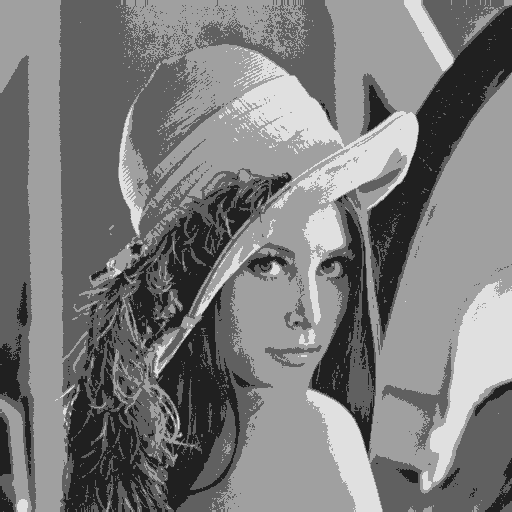
\includegraphics[scale=0.3]{resources/png/naive4.png}
        \end{minipage}\hfill
        \begin{minipage}[b]{0.3\linewidth}
    	    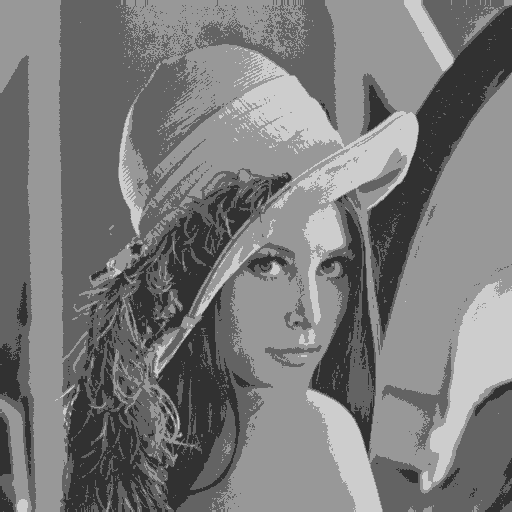
\includegraphics[scale=0.3]{resources/png/greedy4.png}
        \end{minipage}\hfill
        \begin{minipage}[b]{0.3\linewidth}
    	    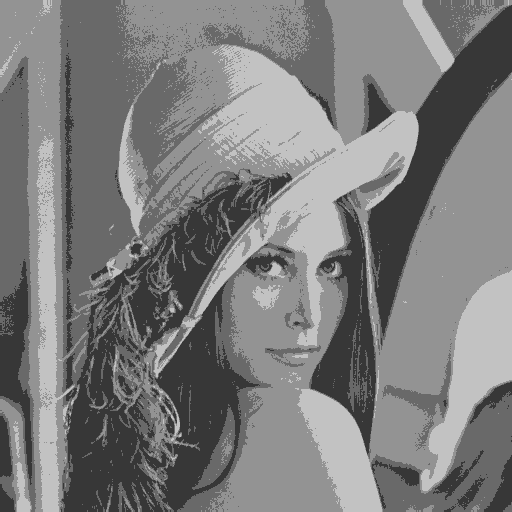
\includegraphics[scale=0.3]{resources/png/dp4.png}
        \end{minipage}
        \caption{Compression sur 4 niveaux par l'approche naïve à gauche, par l'approche gloutonne au centre et par la programmation dynamique à droite.}
    \end{figure}
    
    Sur 4 niveaux, on se rend compte que l'approche dynamique offre plus de contrastes, là où l'approche naïve fournit un résultat plus marqué au moyen de tons de gris plus éloignés les uns des autres, ce qui est moins fidèle à l'image de base. L'approche gloutonne fournit un résultat assez similaire à l'approche par programmation dynamique, mais offre moins de contraste. L'approche par programmation dynamique semble fournir le résultat le plus fidèle à l'original et supprime moins de détails au niveau du visage que l'approche gloutonne.
    
    \subsubsection{Compression sur 10 niveaux}
	\begin{figure}[ht!]
	    \centering
    	\begin{minipage}[b]{0.3\linewidth}
    	    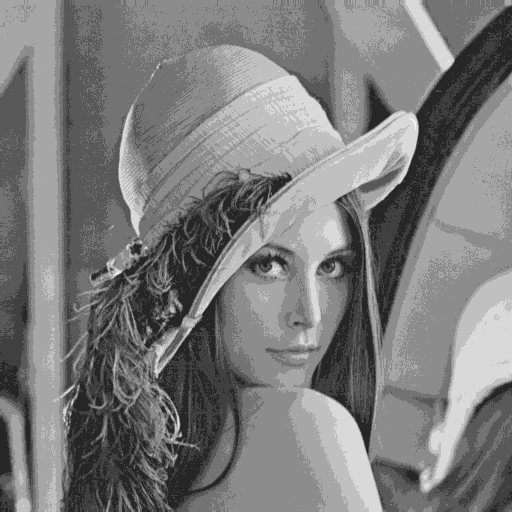
\includegraphics[scale=0.3]{resources/png/naive10.png}
        \end{minipage}\hfill
        \begin{minipage}[b]{0.3\linewidth}
    	    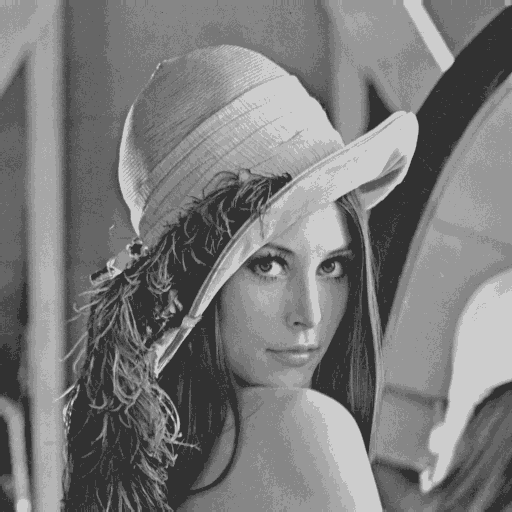
\includegraphics[scale=0.3]{resources/png/greedy10.png}
        \end{minipage}\hfill
        \begin{minipage}[b]{0.3\linewidth}
    	    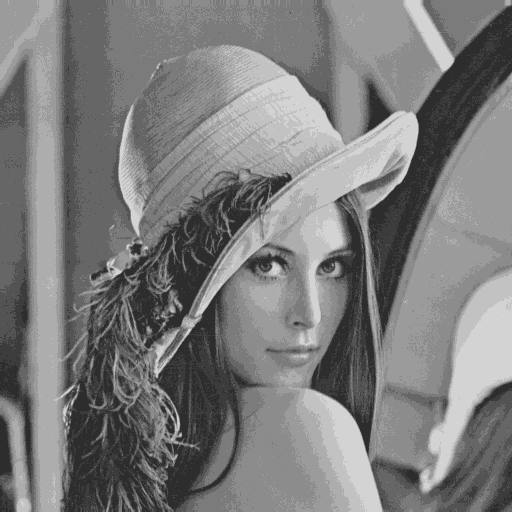
\includegraphics[scale=0.3]{resources/png/dp10.png}
        \end{minipage}
        \caption{Compression sur 10 niveaux par l'approche naïve à gauche, par l'approche gloutonne au centre et par la programmation dynamique à droite.}
    \end{figure}
    
    Sur 10 niveaux, la différence entre les approches reste marquée. L'approche naïve fournit un résultat assez grossier tandis que les deux autres donnent des images plus précises. Au niveau de l'épaule et de l'objet sur la droite, on voit que l'approche DPR est plus précise que son homologue gloutonne.
    \subsubsection{Compression sur 50 niveaux}
	\begin{figure}[ht!]
	    \centering
    	\begin{minipage}[b]{0.3\linewidth}
    	    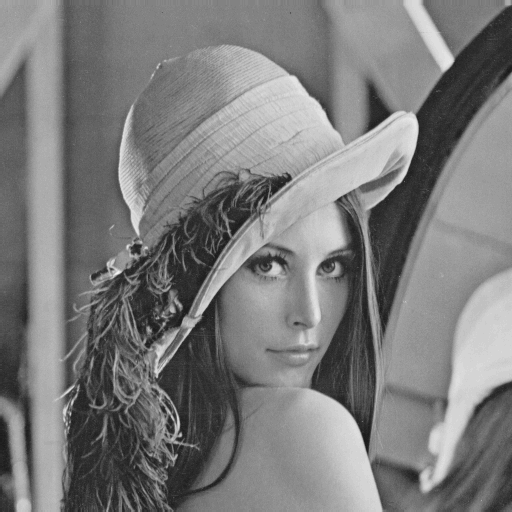
\includegraphics[scale=0.3]{resources/png/naive50.png}
        \end{minipage}\hfill
        \begin{minipage}[b]{0.3\linewidth}
    	    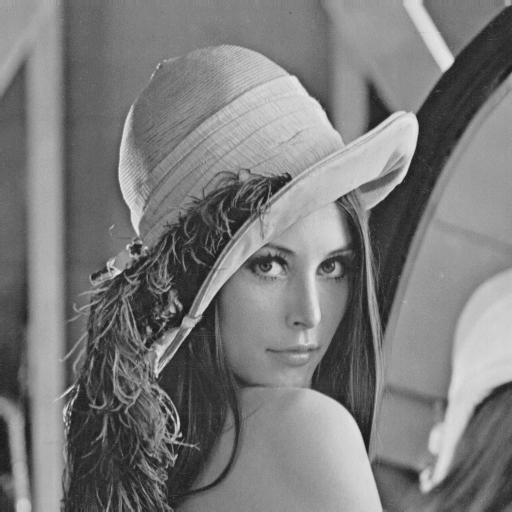
\includegraphics[scale=0.3]{resources/png/greedy50.png}
        \end{minipage}\hfill
        \begin{minipage}[b]{0.3\linewidth}
    	    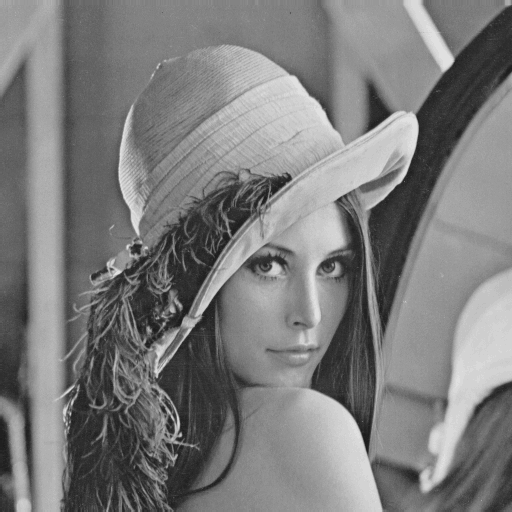
\includegraphics[scale=0.3]{resources/png/dp50.png}
        \end{minipage}
        \caption{Compression sur 50 niveaux par l'approche naïve à gauche, par l'approche gloutonne au centre et par la programmation dynamique à droite.}
    \end{figure}
    
    Sur 50 niveaux, les différences s'amenuisent. Les tons du visage sont peut-être moins marqués sur l'image naïve mais les deux autres sont fortement identiques. Pour de faibles valeurs de k, il est plus intéressant d'utiliser l'approche dynamique mais quand k s'approche de 50, l'approche gloutonne fournit un résultat aussi satisfaisant.
\end{document}
